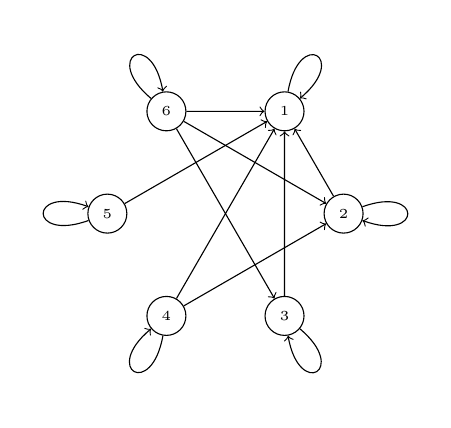
\begin{tikzpicture}[scale=1.5]
  \foreach \i in {1,...,6} {
    \node[circle, draw] (a\i) at (120-\i*60:1) {\tiny \i};
    \draw[->] (a\i) edge [in=100-\i*60, out=140-\i*60,looseness=12] (a\i);
  }
    \draw[->] (a2) edge (a1);
    \draw[->] (a3) edge (a1);
    \draw[->] (a4) edge (a1);
    \draw[->] (a4) edge (a2);
    \draw[->] (a5) edge (a1);
    \draw[->] (a6) edge (a1);
    \draw[->] (a6) edge (a2);
    \draw[->] (a6) edge (a3);
  \end{tikzpicture}